%---------------------------------------------------------------------------------------------------
%		platform.tex
%
%	This file contains the sections that describe available IaaS cloud platform and its main features
%
%	Author: Andrea Meneghinello
% Version: 0.1
%	Table of changes:
%		17/03/2016 -> document definition
%---------------------------------------------------------------------------------------------------
\section{\acs{paas} cloud platforms}
\label{sec:background-cloudPlatform}
In the previous sections we have illustrated what cloud computing is and how it can make resources
available to us through the virtualization technique. 

Now we want to illustrate some of the major \ac{paas} provider competitors in the market. Each one 
has characteristics that differentiate it from the others. In the following section we will see that
some of the major competitors have started the integration of the Docker \ac{api} inside their platforms.

\subsection*{Cloud unit}
\label{sec:background-cloudPlatform-cloudUnit}
CloudUnit \cite{cloudUnitHomepage} is an open-source \ac{paas} for Java applications. It provides an
automated and standardized platform for developers to build and run Java applications, as faster as
possible, and operational to provision and orchestrate environments.

Its main characteristics are:

\begin{itemize}
	\item{\keyword{infrastructure agnostic}: it is able to run on top of any \acs{it} infrastructure
		(\ac{vm}s, bare-metal, public, private and also hybrid cloud, etc.);}
	\item{\keyword{tools}: developers can deploy new or legacy applications without changing any line
		of code and using their preferred tools;}
	\item{\keyword{portability}: it is based on Docker which ensures that deployed applications will
		work seamlessly on any environment;}
	\item{\keyword{open-source}: it is able to eliminate lock-in problem because it is licensed under
		the GNU public license 3.0.}
\end{itemize}

\subsection*{Docker data center}
\label{sec:background-cloudPlatform-dockerDataCentre}
At the end of February Docker announced \cite{dockerDataCentrePresentation} the release of its data-centre
\cite{dockerDataCentre} (shown in Figure \ref{img:background-cloudPlatform-dockerDataCetre}) which
brings containers management and services deployment to the enterprise
with a production ready \ac{caas} that is supported by Docker and hosted locally, behind their firewalls.

The biggest difference between Docker data-centre and other \ac{paas} providers is that Docker \ac{caas}
is an end-to-end fully Docker-native platform. This means that users can utilize the Docker \ac{cli}
and the full set of \acs{api}. The platform is extremely pluggable as they believe in the philosophy of
``batteries included, but swappable.'' Users can simply plug Docker \ac{caas} into their existing
environments, avoiding vendor lock-in.

\begin{figure}
	\centering{}
	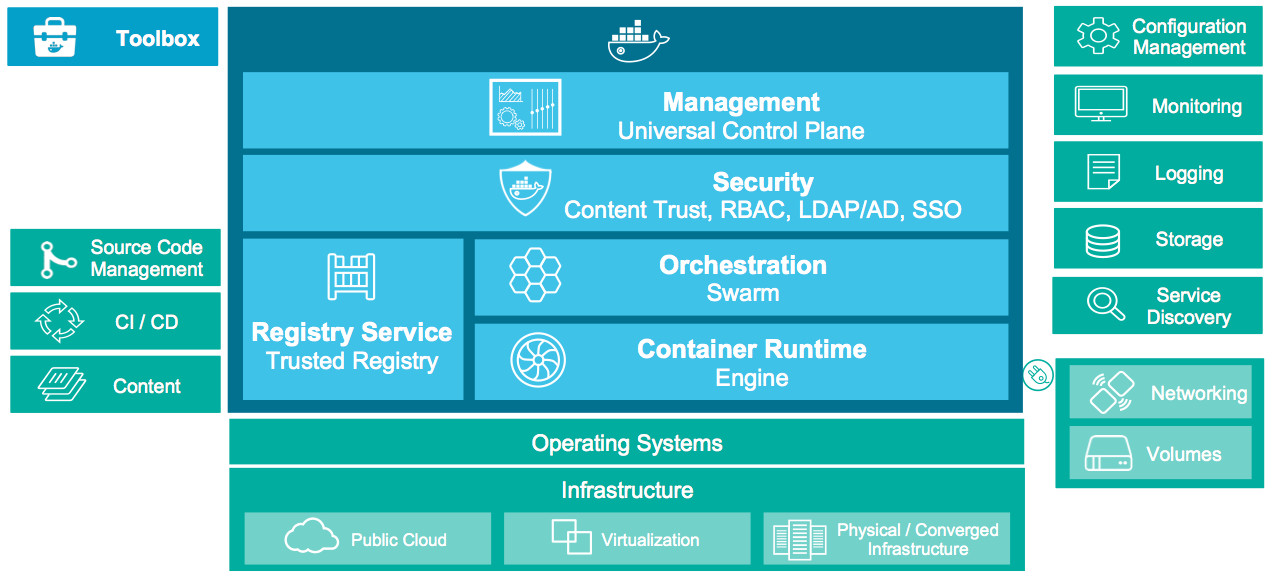
\includegraphics[width=0.65\textwidth]{chapters/background/images/docker-datacentre.png}
	\caption[Docker data-centre architecture]{Docker data-centre architecture \cite{dockerDataCentreArchitecture}.}
	\label{img:background-cloudPlatform-dockerDataCetre}
\end{figure}

\ac{paas} solutions are notorious for locking customers into using a particular infrastructure. They
are often cobbled together solutions that are not natively integrated. For instance, you could use
something like OpenShift, but then your orchestration might be Kubernetes, while also using the open
source Docker engine.